\documentclass[12pt]{article}
\usepackage[margin=2.5cm]{geometry}
\usepackage{enumerate}
\usepackage{amsfonts}
\usepackage{amsmath}
\usepackage{fancyhdr}
\usepackage{amsmath}
\usepackage{amssymb}
\usepackage{amsthm}
\usepackage{mdframed}
\usepackage{graphicx}
\usepackage{subcaption}
\usepackage{adjustbox}
\usepackage{listings}
\usepackage{xcolor}
\usepackage{booktabs}
\usepackage[utf]{kotex}
\usepackage{hyperref}

\definecolor{codegreen}{rgb}{0,0.6,0}
\definecolor{codegray}{rgb}{0.5,0.5,0.5}
\definecolor{codepurple}{rgb}{0.58,0,0.82}
\definecolor{backcolour}{rgb}{0.95,0.95,0.92}

\lstdefinestyle{mystyle}{
    backgroundcolor=\color{backcolour},
    commentstyle=\color{codegreen},
    keywordstyle=\color{magenta},
    numberstyle=\tiny\color{codegray},
    stringstyle=\color{codepurple},
    basicstyle=\ttfamily\footnotesize,
    breakatwhitespace=false,
    breaklines=true,
    captionpos=b,
    keepspaces=true,
    numbers=left,
    numbersep=5pt,
    showspaces=false,
    showstringspaces=false,
    showtabs=false,
    tabsize=1
}

\lstset{style=mystyle}

\pagestyle{fancy}
\renewcommand{\headrulewidth}{0.4pt}
\lhead{CSC 373}
\rhead{Worksheet 3}

\begin{document}
\title{CSC373 Worksheet 3}
\maketitle

\bigskip

Source: \href{http://www.cs.toronto.edu/~denisp/csc373/material.html}{link}

\begin{enumerate}[1.]
    \item \textbf{CLRS 15.2-1:} Find an optimal parenthesization of a matrix-chain product whose sequence of dimension is
    $<5,10,3,12,5,50,6>$

    \item \textbf{CLRS 15.2-2:} Give a recursive algorithm $MATRIX-CHAIN-MULTIPLY(A,s,i,j)$ that actually
    performs the optimal matrix-chain multiplication, given the sequence o matrices $<A_1, A_3, ..., A_n>$,
    the $s$ table computed by $MATRIX-CHAIN-ORDER$, and the indices $i$ and $j$. (The
    initial call would be $MATRIX-CHAIN-MULTIPLY(A,s,1,n)$).

    \item \textbf{CLRS 15.2-5:} Let $R(i,j)$ be the number of times that table entry $m[i,j]$ is referenced
    while computing other table entries in call of $MATRIX-CHAIN-ORDER$. Show that the
    total number of references for the entire table is

    \begin{align*}
    \sum\limits_{i=1}^n \sum\limits_{j=1} R(i,j) &= \frac{n^3 - n}{3}
    \end{align*}

    \item \textbf{CLRS 15.3-2:} Draw the recursion tree for $MERGE-SORT$ procedure from Section 2.3.1 on an
    array of 16 elements. Explain why memoization fails to speed up a good divide-and-conquer algorithm such as $MERGE-SORT$

    \item \textbf{CLRS 15.3-3:} Consider a variant of the matrix-chain multiplication problem in which the goal
    is to parenthesize the seqnce of matrices so as to maximize, rather than minimize the number of scalar multiplications.
    Does this problem exhibit optimal substructure?

    \item \textbf{CLRS 15.3-4:} As stated, in dynamic programming we first solve hte subproblems and then choose which of them
    to use in an optimal solution to the problem. Professor Capulet claims that we do not always need to solve all the subproblems
    in order to find an optimal solution. She suggests that we can find an optimal solution to the matrix chain multiplication problem
    by always choosing the matrix $A_k$ at which to split the subproduct $A_iA_{i+1}...A_j$

    \item \textbf{CLRS 15.4-1:} Determine an LCS of $<1,0,0,1,0,1,0,1>$ and $<0,1,0,1,1,0,1,1,0>$

    \item \textbf{CLRS 15.4-2:} Give pseudocode to reconstruct an LCS from the completed $c$ table
    and the original sequences $X = <x_1,x_2,...,x_m>$ and $Y = <y_1, y_2, ..., Y_n>$ in $O(m+n)$ time,
    without using the $b$ table.

    \item \textbf{CLRS 15.4-6:} Give an $O(n \lg n)$-time algorithm to find the longest monotonically increasing subsequence
    of a seuence of $n$ numbers. (Hint: Observe that the last element of a candidate subseqneuce of length $i$ is at least as
    large as the last element of a candidate subseqneunce of length $i-1$. Maintain candidate subsequences by linking them
    through the input sequence)

    \item \textbf{DPV 6.7:} A sequence is \textit{palindromic} if it is the same
    whether read left to right or right to left. For instance, the sequence

    \begin{align*}
        A,C,G,T,G,T,C,A,A,A,A,T,C,G
    \end{align*}

    has many palindromic subsequences, including $A,C,G,C,A$ and $A,A,A,A$ (on the other hand,
    the subsequence $A,C,T$ is not palindromic). Devise an algorithm that takes a sequence $x[1...n]$
    and returns the (length of the) longest palindromic subsequence. It's running time should be $O(n^2)$.

    \item \textbf{DPV 6.21:} A \textit{vertac cover} of a graph $G = (V,E)$ is a subset of verticies $S \subseteq V$ that includes
    at least one endpoint of every edge in $E$. Give a linear-time algorithm for the following task

    \bigskip

    \textit{Input:} An undirected tree $T = (V,E)$

    \textit{Output:} The size of the smallest vertex cover of $T$

    \bigskip

    For instance, in the following tree, possible vertex covers include $\{A,B,C,D,E,F,G\}$
    and $\{A,C,D,F\}$ but not $\{C,E,F\}$. The smallest vertex cover has size 3: $\{B,E,G\}$.

    \bigskip

    \begin{center}
    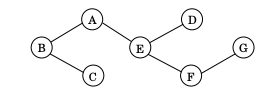
\includegraphics[width=0.7\linewidth]{images/worksheet_3_1.png}
    \end{center}
\end{enumerate}

\end{document}